\documentclass{article}\usepackage[]{graphicx}\usepackage[]{color}
%% maxwidth is the original width if it is less than linewidth
%% otherwise use linewidth (to make sure the graphics do not exceed the margin)
\makeatletter
\def\maxwidth{ %
  \ifdim\Gin@nat@width>\linewidth
    \linewidth
  \else
    \Gin@nat@width
  \fi
}
\makeatother

\definecolor{fgcolor}{rgb}{0.345, 0.345, 0.345}
\newcommand{\hlnum}[1]{\textcolor[rgb]{0.686,0.059,0.569}{#1}}%
\newcommand{\hlstr}[1]{\textcolor[rgb]{0.192,0.494,0.8}{#1}}%
\newcommand{\hlcom}[1]{\textcolor[rgb]{0.678,0.584,0.686}{\textit{#1}}}%
\newcommand{\hlopt}[1]{\textcolor[rgb]{0,0,0}{#1}}%
\newcommand{\hlstd}[1]{\textcolor[rgb]{0.345,0.345,0.345}{#1}}%
\newcommand{\hlkwa}[1]{\textcolor[rgb]{0.161,0.373,0.58}{\textbf{#1}}}%
\newcommand{\hlkwb}[1]{\textcolor[rgb]{0.69,0.353,0.396}{#1}}%
\newcommand{\hlkwc}[1]{\textcolor[rgb]{0.333,0.667,0.333}{#1}}%
\newcommand{\hlkwd}[1]{\textcolor[rgb]{0.737,0.353,0.396}{\textbf{#1}}}%

\usepackage{framed}
\makeatletter
\newenvironment{kframe}{%
 \def\at@end@of@kframe{}%
 \ifinner\ifhmode%
  \def\at@end@of@kframe{\end{minipage}}%
  \begin{minipage}{\columnwidth}%
 \fi\fi%
 \def\FrameCommand##1{\hskip\@totalleftmargin \hskip-\fboxsep
 \colorbox{shadecolor}{##1}\hskip-\fboxsep
     % There is no \\@totalrightmargin, so:
     \hskip-\linewidth \hskip-\@totalleftmargin \hskip\columnwidth}%
 \MakeFramed {\advance\hsize-\width
   \@totalleftmargin\z@ \linewidth\hsize
   \@setminipage}}%
 {\par\unskip\endMakeFramed%
 \at@end@of@kframe}
\makeatother

\definecolor{shadecolor}{rgb}{.97, .97, .97}
\definecolor{messagecolor}{rgb}{0, 0, 0}
\definecolor{warningcolor}{rgb}{1, 0, 1}
\definecolor{errorcolor}{rgb}{1, 0, 0}
\newenvironment{knitrout}{}{} % an empty environment to be redefined in TeX

\usepackage{alltt}
\usepackage{amsmath}
\usepackage{lscape}
\IfFileExists{upquote.sty}{\usepackage{upquote}}{}
\begin{document}






\begin{knitrout}
\definecolor{shadecolor}{rgb}{0.969, 0.969, 0.969}\color{fgcolor}\begin{kframe}
\begin{alltt}
\hlcom{# xy = matrix(runif(10000), ncol = 2)}
\hlcom{# xy = xy[xy[,1] < 0.1 | xy[,2] < 0.1,]}
\hlcom{# xy = xy %*% matrix(c(1, 0.4, 0.4, 1), ncol = 2)}
\hlcom{# xy = xy[xy[,1] <= 1 & xy[,2] <= 1,]}

\hlstd{xyc} \hlkwb{=} \hlkwd{read.csv}\hlstd{(}\hlstr{"synthetic_data.csv"}\hlstd{)}
\hlstd{xy} \hlkwb{=} \hlstd{xyc[,}\hlnum{1}\hlopt{:}\hlnum{2}\hlstd{]}

\hlkwd{set.seed}\hlstd{(}\hlnum{1234}\hlstd{)}
\hlstd{subset} \hlkwb{=} \hlkwd{sample.int}\hlstd{(}\hlkwd{nrow}\hlstd{(xy),} \hlnum{300}\hlstd{)}

\hlkwd{library}\hlstd{(fastICA)}
\hlkwd{library}\hlstd{(NMF)}
\end{alltt}


{\ttfamily\noindent\itshape\color{messagecolor}{\#\# Loading required package: methods\\\#\# Loading required package: pkgmaker\\\#\# Loading required package: registry\\\#\# Loading required package: rngtools\\\#\# Loading required package: cluster\\\#\# NMF - BioConductor layer [OK] | Shared memory capabilities [OK] | Cores 2/2}}\begin{alltt}
\hlstd{fit.pca} \hlkwb{=} \hlkwd{prcomp}\hlstd{(xy,} \hlkwc{center} \hlstd{=} \hlnum{TRUE}\hlstd{,} \hlkwc{scale} \hlstd{=} \hlnum{FALSE}\hlstd{)}

\hlstd{temp} \hlkwb{=} \hlkwd{replicate}\hlstd{(}\hlnum{1000}\hlstd{,} \hlkwd{fastICA}\hlstd{(xy,} \hlnum{2}\hlstd{,} \hlkwc{method} \hlstd{=} \hlstr{"C"}\hlstd{),} \hlkwc{simplify} \hlstd{=} \hlnum{FALSE}\hlstd{)}
\hlstd{temp2} \hlkwb{=} \hlkwd{sapply}\hlstd{(temp,} \hlkwa{function}\hlstd{(}\hlkwc{x}\hlstd{)} \hlkwd{shapiro.test}\hlstd{(x}\hlopt{$}\hlstd{S)}\hlopt{$}\hlstd{statistic)}
\hlstd{fit.ica} \hlkwb{=} \hlstd{temp[[}\hlkwd{which.max}\hlstd{(temp2)]]}

\hlstd{fit.nmf} \hlkwb{=} \hlkwd{nmf}\hlstd{(}\hlkwd{t}\hlstd{(xy[subset,]),} \hlkwc{rank} \hlstd{=} \hlnum{2}\hlstd{,} \hlkwc{nrun} \hlstd{=} \hlnum{20}\hlstd{,} \hlkwc{method} \hlstd{=} \hlstr{"snmf/r"}\hlstd{)}
\end{alltt}
\end{kframe}
\end{knitrout}



\begin{knitrout}
\definecolor{shadecolor}{rgb}{0.969, 0.969, 0.969}\color{fgcolor}\begin{kframe}
\begin{alltt}
\hlkwd{library}\hlstd{(NMF)}
\end{alltt}


{\ttfamily\noindent\itshape\color{messagecolor}{\#\# Loading required package: methods\\\#\# Loading required package: pkgmaker\\\#\# Loading required package: registry\\\#\# Loading required package: rngtools\\\#\# Loading required package: cluster\\\#\# NMF - BioConductor layer [OK] | Shared memory capabilities [OK] | Cores 3/4}}\begin{alltt}
\hlkwd{library}\hlstd{(RColorBrewer)}
\hlkwd{library}\hlstd{(ggplot2)}
\hlkwd{library}\hlstd{(grid)}

\hlstd{pal} \hlkwb{=} \hlkwd{brewer.pal}\hlstd{(}\hlnum{3}\hlstd{,} \hlstr{"Set2"}\hlstd{)[}\hlkwd{c}\hlstd{(}\hlnum{2}\hlstd{,} \hlnum{3}\hlstd{,} \hlnum{1}\hlstd{)]}
\hlstd{pal} \hlkwb{=} \hlkwd{sapply}\hlstd{(pal,} \hlkwa{function}\hlstd{(}\hlkwc{col}\hlstd{)} \hlkwd{do.call}\hlstd{(rgb,} \hlkwd{c}\hlstd{(}\hlkwd{as.list}\hlstd{(}\hlkwd{col2rgb}\hlstd{(col)}\hlopt{/}\hlnum{255}\hlstd{),} \hlkwc{alpha} \hlstd{=} \hlnum{0.5}\hlstd{)))}
\hlstd{syms} \hlkwb{=} \hlkwd{c}\hlstd{(}\hlnum{19}\hlstd{,} \hlnum{4}\hlstd{,} \hlnum{21}\hlstd{)}
\hlstd{col} \hlkwb{=} \hlstd{pal[xyc[,}\hlnum{3}\hlstd{]]}
\hlstd{pch} \hlkwb{=} \hlstd{syms[xyc[,}\hlnum{3}\hlstd{]]}

\hlcom{# plot(0 ~ 0, type = "n", xlab = "Gene 1", ylab = "Gene 2", xlim = c(0, 1), ylim = c(0, 1), xaxt = "n", yaxt = "n", asp = 1)}
\hlcom{# # arrows(}
\hlcom{# # 	x0 = c(0, 0), }
\hlcom{# # 	y0 = c(0, 0), }
\hlcom{# # 	x1 = c(0.5, 1), }
\hlcom{# # 	y1 = c(1, 0.45), }
\hlcom{# # 	col = "lightgrey", lwd = 5)}
\hlcom{# points(xy[subset,1], xy[subset,2], col = "black", pch = pch[subset])}
\hlcom{# legend("topright", legend = c("State A", "State B", "Transition State"), pch = syms[c(3, 1, 2)], inset = 0.05)}

\hlcom{# for (spec in list(list(fit.pca$rotation, colMeans(xy)), list(fit.ica$A, colMeans(xy)), list(basis(fit.nmf), c(0, 0))))}
\hlcom{# \{}
\hlcom{# 	plot(xy[subset,1], xy[subset,2], col = rgb(0, 0, 0, 0.5), pch = pch[subset], xlab = "", ylab = "", xlim = c(0, 1), ylim = c(0, 1), xaxt = "n", yaxt = "n", asp = 1)}
\hlcom{# 	temp = spec[[1]]}
\hlcom{# 	temp = t(t(temp) / sqrt(colSums(temp^2)) / 2)}
\hlcom{# 	arrows(}
\hlcom{# 		x0 = spec[[2]][1], }
\hlcom{# 		y0 = spec[[2]][2], }
\hlcom{# 		x1 = temp[1,] + spec[[2]][1], }
\hlcom{# 		y1 = temp[2,] + spec[[2]][2], }
\hlcom{# 		col = "black", lwd = 5)}
\hlcom{# \}}

\hlkwd{ggplot}\hlstd{(}\hlkwd{data.frame}\hlstd{(}\hlkwc{x} \hlstd{= xyc[,}\hlnum{1}\hlstd{],} \hlkwc{y} \hlstd{= xyc[,}\hlnum{2}\hlstd{],} \hlkwc{State} \hlstd{=} \hlkwd{as.factor}\hlstd{(}\hlkwd{c}\hlstd{(}\hlstr{"B"}\hlstd{,} \hlstr{"Transition"}\hlstd{,} \hlstr{"A"}\hlstd{)[xyc[,}\hlnum{3}\hlstd{]]))[subset,],} \hlkwd{aes}\hlstd{(x, y,} \hlkwc{pch} \hlstd{= State))} \hlopt{+}
        \hlkwd{geom_point}\hlstd{()} \hlopt{+}
        \hlkwd{coord_fixed}\hlstd{(}\hlkwc{xlim} \hlstd{=} \hlkwd{c}\hlstd{(}\hlnum{0}\hlstd{,} \hlnum{1}\hlstd{),} \hlkwc{ylim} \hlstd{=} \hlkwd{c}\hlstd{(}\hlnum{0}\hlstd{,} \hlnum{1}\hlstd{),} \hlkwc{ratio} \hlstd{=} \hlnum{1}\hlstd{)} \hlopt{+}
        \hlkwd{theme_bw}\hlstd{()} \hlopt{+}
        \hlkwd{xlab}\hlstd{(}\hlstr{"Gene 1"}\hlstd{)} \hlopt{+} \hlkwd{ylab}\hlstd{(}\hlstr{"Gene 2"}\hlstd{)} \hlopt{+}
        \hlkwd{theme}\hlstd{(}\hlkwc{axis.ticks} \hlstd{=} \hlkwd{element_blank}\hlstd{(),} \hlkwc{axis.text.x} \hlstd{=} \hlkwd{element_blank}\hlstd{(),} \hlkwc{axis.text.y} \hlstd{=} \hlkwd{element_blank}\hlstd{())} \hlopt{+}
        \hlkwd{scale_shape_manual}\hlstd{(}\hlkwc{values} \hlstd{=} \hlkwd{c}\hlstd{(}\hlnum{21}\hlstd{,} \hlnum{19}\hlstd{,} \hlnum{4}\hlstd{))}
\end{alltt}
\end{kframe}

{\centering 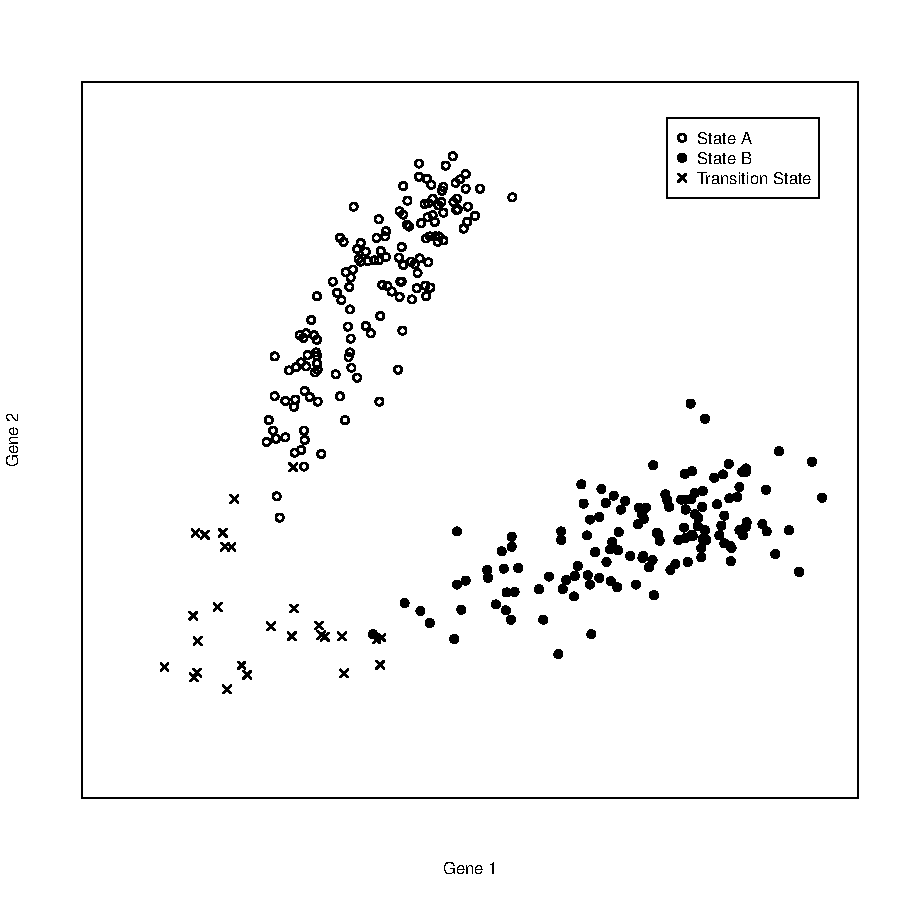
\includegraphics[width=\maxwidth]{figure/plots-1} 

}



\end{knitrout}


\begin{knitrout}
\definecolor{shadecolor}{rgb}{0.969, 0.969, 0.969}\color{fgcolor}\begin{kframe}
\begin{alltt}
\hlstd{baseplot} \hlkwb{=} \hlkwd{ggplot}\hlstd{(}\hlkwd{data.frame}\hlstd{(}\hlkwc{x} \hlstd{= xyc[,}\hlnum{1}\hlstd{],} \hlkwc{y} \hlstd{= xyc[,}\hlnum{2}\hlstd{],} \hlkwc{State} \hlstd{=} \hlkwd{as.factor}\hlstd{(}\hlkwd{c}\hlstd{(}\hlstr{"B"}\hlstd{,} \hlstr{"Transition"}\hlstd{,} \hlstr{"A"}\hlstd{)[xyc[,}\hlnum{3}\hlstd{]]))[subset,],} \hlkwd{aes}\hlstd{(x, y,} \hlkwc{pch} \hlstd{= State))} \hlopt{+}
        \hlkwd{geom_point}\hlstd{(}\hlkwc{col} \hlstd{=} \hlstr{"darkgrey"}\hlstd{)} \hlopt{+}
        \hlkwd{coord_fixed}\hlstd{(}\hlkwc{xlim} \hlstd{=} \hlkwd{c}\hlstd{(}\hlnum{0}\hlstd{,} \hlnum{1}\hlstd{),} \hlkwc{ylim} \hlstd{=} \hlkwd{c}\hlstd{(}\hlnum{0}\hlstd{,} \hlnum{1}\hlstd{),} \hlkwc{ratio} \hlstd{=} \hlnum{1}\hlstd{)} \hlopt{+}
        \hlkwd{theme_bw}\hlstd{()} \hlopt{+}
        \hlkwd{theme}\hlstd{(}\hlkwc{axis.ticks} \hlstd{=} \hlkwd{element_blank}\hlstd{(),} \hlkwc{axis.text.x} \hlstd{=} \hlkwd{element_blank}\hlstd{(),} \hlkwc{axis.text.y} \hlstd{=} \hlkwd{element_blank}\hlstd{(),} \hlkwc{axis.title.x} \hlstd{=} \hlkwd{element_blank}\hlstd{(),} \hlkwc{axis.title.y} \hlstd{=} \hlkwd{element_blank}\hlstd{())} \hlopt{+}
        \hlkwd{scale_shape_manual}\hlstd{(}\hlkwc{values} \hlstd{=} \hlkwd{c}\hlstd{(}\hlnum{21}\hlstd{,} \hlnum{19}\hlstd{,} \hlnum{4}\hlstd{))} \hlopt{+}
        \hlkwd{theme}\hlstd{(}\hlkwc{legend.position}\hlstd{=}\hlstr{"none"}\hlstd{)}


\hlkwa{for} \hlstd{(spec} \hlkwa{in} \hlkwd{list}\hlstd{(}\hlkwd{list}\hlstd{(fit.pca}\hlopt{$}\hlstd{rotation,} \hlkwd{colMeans}\hlstd{(xy)),} \hlkwd{list}\hlstd{(fit.ica}\hlopt{$}\hlstd{A,} \hlkwd{colMeans}\hlstd{(xy)),} \hlkwd{list}\hlstd{(}\hlkwd{basis}\hlstd{(fit.nmf),} \hlkwd{c}\hlstd{(}\hlnum{0}\hlstd{,} \hlnum{0}\hlstd{))))}
\hlstd{\{}
        \hlstd{temp} \hlkwb{=} \hlstd{spec[[}\hlnum{1}\hlstd{]]}
        \hlstd{temp} \hlkwb{=} \hlkwd{t}\hlstd{(}\hlkwd{t}\hlstd{(temp)} \hlopt{/} \hlkwd{sqrt}\hlstd{(}\hlkwd{colSums}\hlstd{(temp}\hlopt{^}\hlnum{2}\hlstd{))} \hlopt{/} \hlnum{2}\hlstd{)}
        \hlstd{thisplot} \hlkwb{=} \hlstd{baseplot} \hlopt{+}
                \hlkwd{geom_segment}\hlstd{(}\hlkwc{x} \hlstd{= spec[[}\hlnum{2}\hlstd{]][}\hlnum{1}\hlstd{],} \hlkwc{xend} \hlstd{= temp[}\hlnum{1}\hlstd{,}\hlnum{1}\hlstd{]} \hlopt{+} \hlstd{spec[[}\hlnum{2}\hlstd{]][}\hlnum{1}\hlstd{],} \hlkwc{y} \hlstd{= spec[[}\hlnum{2}\hlstd{]][}\hlnum{2}\hlstd{],} \hlkwc{yend} \hlstd{= temp[}\hlnum{2}\hlstd{,}\hlnum{1}\hlstd{]} \hlopt{+} \hlstd{spec[[}\hlnum{2}\hlstd{]][}\hlnum{2}\hlstd{],}
                        \hlkwc{arrow} \hlstd{=} \hlkwd{arrow}\hlstd{(}\hlkwc{length} \hlstd{=} \hlkwd{unit}\hlstd{(}\hlnum{0.5}\hlstd{,} \hlstr{"cm"}\hlstd{)),} \hlkwc{size} \hlstd{=} \hlnum{1.5}\hlstd{,} \hlkwc{colour} \hlstd{=} \hlstr{"black"}\hlstd{,} \hlkwc{alpha} \hlstd{=} \hlnum{0.4}\hlstd{)} \hlopt{+}
                \hlkwd{geom_segment}\hlstd{(}\hlkwc{x} \hlstd{= spec[[}\hlnum{2}\hlstd{]][}\hlnum{1}\hlstd{],} \hlkwc{xend} \hlstd{= temp[}\hlnum{1}\hlstd{,}\hlnum{2}\hlstd{]} \hlopt{+} \hlstd{spec[[}\hlnum{2}\hlstd{]][}\hlnum{1}\hlstd{],} \hlkwc{y} \hlstd{= spec[[}\hlnum{2}\hlstd{]][}\hlnum{2}\hlstd{],} \hlkwc{yend} \hlstd{= temp[}\hlnum{2}\hlstd{,}\hlnum{2}\hlstd{]} \hlopt{+} \hlstd{spec[[}\hlnum{2}\hlstd{]][}\hlnum{2}\hlstd{],}
                        \hlkwc{arrow} \hlstd{=} \hlkwd{arrow}\hlstd{(}\hlkwc{length} \hlstd{=} \hlkwd{unit}\hlstd{(}\hlnum{0.5}\hlstd{,} \hlstr{"cm"}\hlstd{)),} \hlkwc{size} \hlstd{=} \hlnum{1.5}\hlstd{,} \hlkwc{colour} \hlstd{=} \hlstr{"black"}\hlstd{,} \hlkwc{alpha} \hlstd{=} \hlnum{0.4}\hlstd{)}
        \hlkwd{print}\hlstd{(thisplot)}
\hlstd{\}}
\end{alltt}
\end{kframe}

{\centering 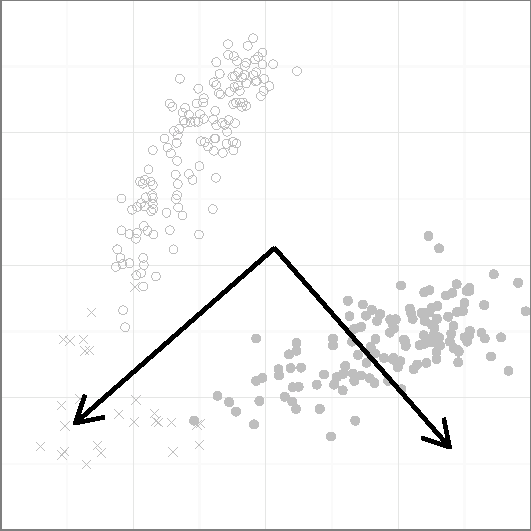
\includegraphics[width=\maxwidth]{figure/smallplots-1} 

}




{\centering 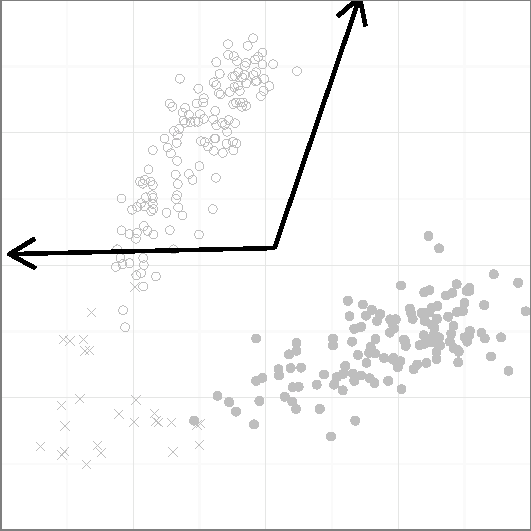
\includegraphics[width=\maxwidth]{figure/smallplots-2} 

}




{\centering 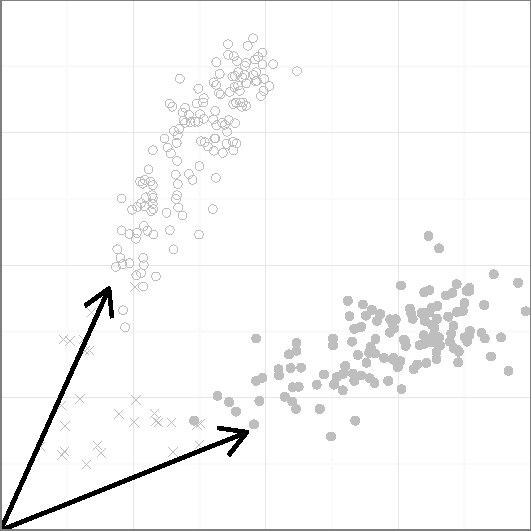
\includegraphics[width=\maxwidth]{figure/smallplots-3} 

}



\end{knitrout}

\end{document}
